

\documentclass[10pt,onecolumn]{lab}
%
% All KJN's macros and goodies (some shameless borrowing from SPL)
\usepackage{KJN}


%\usepackage[hyphens]{url}

%
% PDF Info
%
\ifpdf
\pdfinfo{
/Title (SOFTWARE ENGINEERING PROJECT: STUDENTS MARKS/RECORDS MANAGEMENT SOFTWARE)
/Author (Khosa Masana (559990), Sanele Gcaba(459380), Tshegofatso Misapitso (600313), Londiwe Ngema (448871) )
/ModDate (D:200510121530)
/Subject (ELEN417/455 Paper Format, 2005)
/Keywords (ELEN417, ELEN455, paper, instructions, style guidelines, laboratory project)
}
\fi

%%%%%%%%%%%%%%%%%%%%%%%%%%%%%%%%%%%%%%%%%%%%%%%%%%%%%%%%%%%%%%%%%%%%%%%%%%%%%%%
\begin{document}

\begin{titlepage}

\newcommand{\HRule}{\rule{\linewidth}{0.5mm}} % Defines a new command for the horizontal lines, change thickness here

\center % Center everything on the page
{\small School$\;$of$\;$Electrical$\;$and$\;$Information$\;$Engineering,$\;$University of$\;$the$\;$Witwatersrand,$\;$Private$\;$Bag$\;$3,$\;$2050,$\;$Johannesburg,$\;$South$\;$Africa}\\[1.5cm] % Name of your university/college

\textsc{ELEN 4009 - Software Engineering}\\[0.5cm] % Major heading such as course name

\HRule \\[0.4cm]
{ \large \bfseries Student Marks/Records Management Software - Requirements Gathering}\\[0.4cm] % Title of your document
\HRule \\[1.5cm]

 \large

\textbf{Project Team :}
Khosa$\;$Masana$\;$(559990),
Sanele$\;$Gcaba$\;$(459380),
Tshegofatso$\;$Misapitso$\;$(600313) and
Londiwe$\;$Ngema$\;$(448871)


{\large \today}\\[3cm] % Date, change the \today to a set date if you want to be precise

%\includegraphics{Logo}\\[1cm] % Include a department/university logo - this will require the graphicx package

\vfill % Fill the rest of the page with whitespace

\end{titlepage}

\pagestyle{plain}.
\pagenumbering{roman} 
\tableofcontents 



\newpage

\section*{Document Status Sheet}

\begin{center}
    \begin{tabular}{ | p{5cm} | p{7cm} |}
\hline
\textbf{Document Title}& Software Requirements\\ \hline
\textbf{Authors} & M.$\;$Khosa, S.$\;$Gcaba, T.$\;$Misapitso, L.$\;$Ngema \\ \hline
\textbf{Version} & 0.01 \\ \hline
\textbf{Document Status} & Draft  \\ \hline

    \end{tabular}
\end{center}


\begin{center}
    \begin{tabular}{ | p{2cm} | p{3cm} | p{5cm} | p{5cm} |}
    \hline
    \textbf{Version}& \textbf{Date}& \textbf{Author(s)} & \textbf{Summary} \\ \hline
    0.0.1 & 25-02-2016 & M.$\;$Khosa, S.$\;$Gcaba, T.$\;$Misapitso, L.$\;$Ngema& Document Creation. \\ \hline

    \end{tabular}
\end{center}

\newpage


%%%%%%%%%%%%%%%%%%%%%%%%%%%%%%%%%%%%%%%%%%%%%%%%%%%%%%%%%%%%%%%%%%%%%%%%%%%%%%%
%
\pagestyle{plain}.
\pagenumbering{arabic} 
\section{Introduction}

\subsection{Methodology}

The System Development Life Cycle (SDLC) methodology to be used for the project follows the Agile Model, this models breaks down the product into a cycle, it quickly delivers a working product and is a more realistic methodology. Ongoing releases are produced with small incremental changes and it depends heavily on customer interaction \cite{ref7}. Specifically the Scrum Agile Model will be adopted for the project, as figure 1 below shows, Scrum comprises of short sprints and it enables the software team to be able to prioritize on what matters most. It is basically about delivering more often and getting feedback that is regularly responded to \cite{ref8}.           

\subsection{Purpose}

The purpose of this document is to present a detailed description of the requirements for the student marks/record system (SMMS). It will state the purpose and features of the system, the interfaces of the system, what the system will do, the limitations under which it must operate, define inputs and the expected reaction of the system (that is the outputs of the system). 

Student Marks/Records Management Software provides online services to students and allows staff the rights of editing course marks on the system. It is a convenient way for students to have access to their marks in a safe and confidential way as opposed to accessing them on notice boards where everyone else can publicly see them

\subsection{Project Scope}
\begin{itemize}

\item There are three basic users of the system - Students,  Staff (Lectures) and Admin.
\item The primary function of the application is to allow students to log-in using their details (Student number and password) and be able to access and view their course marks as per requested year of study and courses registered for.
\item The system database stores user profiles and student marks records.
\item The program should have domains assigned by Admin i.e. Staff members can be able to access and edit the database while Students can only view their individual marks. The system would be accessed online via a Browser and a Smart-phone App.
\item Staff log-in using a staff number and password gives rights of editing student records through the student database.
\item The students will be able select the academic year which they require marks for and the specific courses, course code, mark and symbol will be
 displayed to them through a user interface.
\item Admin can add/delete users, grant editing and viewing permission to staff and only viewing rights to students.  

\end{itemize}
\subsection{List of Definitions and abbreviations}

\subsubsection{Definitions}
\begin{center}
    \begin{tabular}{ | p{3cm} | p{9cm} |}
\hline
\textbf{Term}& \textbf{Definition}\\ \hline
 Database & A collection of records stored within the system \\ \hline
 Table & A collection of related data consisting of columns and rows \\ \hline   
     \end{tabular}
\end{center}

\subsubsection{Abbreviations}~\\

\textbf{SMMS} - Student Marks/record management system

\textbf{HTTP} - Hypertext Transfer Protocol

\textbf{HTML} - HyperText Markup Language

\textbf{RDBMS} - Relational Database Management System

\textbf{SQL} - Structured Query Language

%%%%%%%%%%%%%%%%%%%%%%%%%%%%%%%%%%%%%%%%%%%%%%%%%%%%%%%%%%%%%%%%%%%%%%%%%%%%%%%
%
\subsection{Tools used}
\textbf{Web server} - Apache2

The Apache web server is the worlds most used web server software program, it uses HTTP to serve files that form web pages to users in response to their requests. It is an open source program \cite{ref5, ref6}. 

\textbf{Development tools (Front-End)} - HTML, CSS and Javascript

\textbf{Development tools (Back-End)} - PHP 

PHP is a server scripting language, it is widely used, free, and efficient tool.

\textbf{Database Platform} - MySQL and PHPmyadmin 

MySQL is an open-source RDBMS, it stores data in tables and PHPmyadmin is a graphical tool intended to handle administration of MySQL over the web.   
\section{Expanded Description of the project}

The software system will follow a Two-Tier Architecture due to its ease of use and maintainability as compared to a Three-Tier Architecture. However, the performance of a Two-Tier Architecture slows down with an increase in users \cite{ref3}, hence a Three-Tier Architecture will be implemented with an increase of the number of users. Figure 1 below shows the Two-Tier Architecture.   
\begin{center}
\begin{figure}[h]
\centering
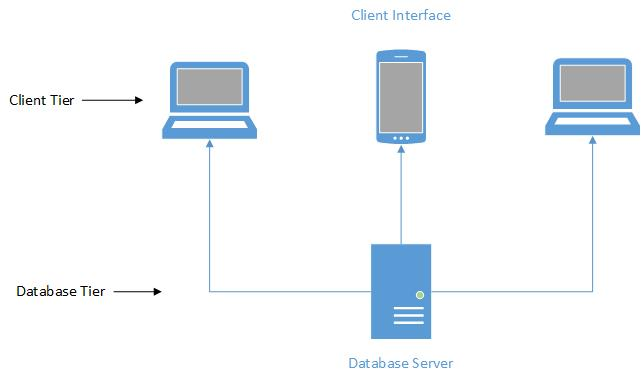
\includegraphics[width=10cm]{Two-Tier}
\caption{Two-Tier Software Architecture}
\end{figure}
\end{center}


A Two-Tier Architecture is a software architecture where the interface runs on client and the data layer is stored on a server\cite{ref4}.
\subsection{Front-End}

Khosa Masana (559990) and Londiwe Ngema (448871) are going to be responsible for the design, development and documentation of the front end (user interface).

Both the user interface of the browser and the smart-phone app are going to be designed using HTML5, CSS and JavaScript. The user interface will offer a platform whereby the users are going to interact with the server. The users (i.e students and staff) will be prompted for a student/staff number and a password to view or change the results. Only the staff members (lecturers) will be given the right to change the results, students can only view the results. Validation of credentials will be done in Javascript before they are submitted to the server.  

\subsubsection{\textbf{System Input and Output:}} 
 
With the student number, password and year entered as an input, the relevant information (results) of that particular student and the particular year will be searched from the server and displayed to the student. Results (Output) will be displayed in a form of a table with course name, course code, results and a symbol as columns. PHP will be used to link the back-end and front-end

\subsection{Back-End}
Sanele Gcaba (459380) and Tshegofatso Misapitso (600313)  are going to be responsible for the design, development and documentation of the back-end (Server and Database).

The back-end:
The proposed design of the back-end is to include a Linux Apache MySQL PHP(LAMP) installation.

The Linux operating system is chosen for the server to run on because of its Stability, Security and Cost of operation \cite{ref1}.   
As a result Linux Mint operating system was chosen.
The Linux is Just the base of the project that will allow the server to run off. The server proposed is an Apache server. This server is chosen because it is easy to install and operate. Apache will provide a secure, efficient and extensible server that provides HTTP services.
The project requires that data is stored and later on read from. There is multiple datasets that need to be considered: for example multiple students that may be doing multiple courses and as a result a need for storing this data. MySQL was chosen because it is an open source database and large companies use it to save money and time powering their high volume websites \cite{ref2}.

PHP is  selected as a server the scripting language. This is chosen because of the simplicity of the language and in addition JavaScript can be used to do client side validation to avoid overloading the server with server side validation. Validation would be necessary for authentication. 

PHPMyadmin may be used in order to get a visual look of the database instead of having to type out queries in order to check that the data one expects to be in the database is actually in the database. 
Interacting: the client tries logging in:

\begin{itemize}
\item Client enters credentials, these credentials get validated ‘onsubmit’.
\item If the credentials are correct: a PHP script is used to determine if the user is a  student or staff member.
\item If the user is a student then the student will only have certain privileges such as reading from the database only.
\item If the user is an administrator or a staff member then they may be allowed to have different privileges to edit the database: such as alter student results and add new student onto the database.
\end{itemize}

\section{Specific Requirements}

\subsection{UML Activity Diagram}

Figure 2 Shows the UML activity diagram of the how the software should work. As shown in the UML activity diagram, the user will first be ask to enter a user-name and a password. This is done to keep track of the type of user who will be interacting with the software i.e student, staff and admin. Each type of user will be given different rights to interact with the server as shown in the UML diagram. Students are only allowed to view the results, staff is allowed to change marks or add results and the administrator will be responsible of adding or removing users.   

\begin{center}
\begin{figure}[h]
\centering
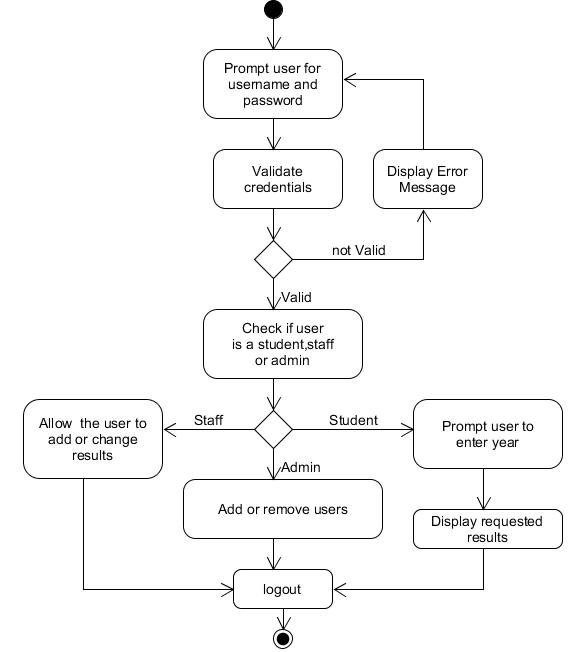
\includegraphics[trim={0cm 0 0 0},clip]{UML-Activity}
\caption{UML Activity Diagram}
\end{figure}
\end{center}

\subsection{Use Case Reports}
Since we have only three users of the software, namely student, staff and administrator, three use case reports have been made for each user. 
 

\clearpage
\subsubsection{Student Use-Case Report}$\;\;\;\;\;\;\;\;\;\;\;\;\;\;\;\;\;\;\;\;\;\;\;$

A use case report for a student is shown in Figure 3.
\begin{center}
\begin{figure}[h]
\centering
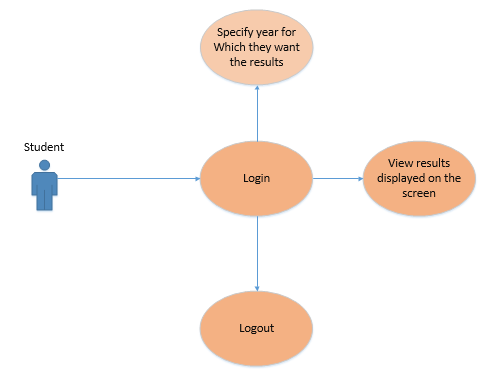
\includegraphics[trim={0cm 0cm 0cm 0cm },clip,scale = 1.1]{StudentUsecase}
\caption{Use Case Diagram For Student}
\end{figure}
\end{center}



\begin{center}
    \begin{tabular}{ | p{2cm} | p{10cm}| }
    \hline
    \textbf{Use case}& \textbf{Description} \\ \hline
    login & The student need to sign in in order to view the results \\ \hline
    Key in Year & The student must be able to specify the year which they need the results for  \\ \hline
    Display results & The student must be able to view the results displayed on the screen \\ \hline
    Logout          & The student must be able to logout  \\ \hline

    \end{tabular}
\end{center}





\clearpage
\subsubsection{Staff Use-Case Report}$\;\;\;\;\;\;\;\;\;\;\;\;\;\;\;\;\;\;\;\;\;\;\;$

A use case report for staff is shown in Figure 4.
\begin{center}
\begin{figure}[h]
\centering
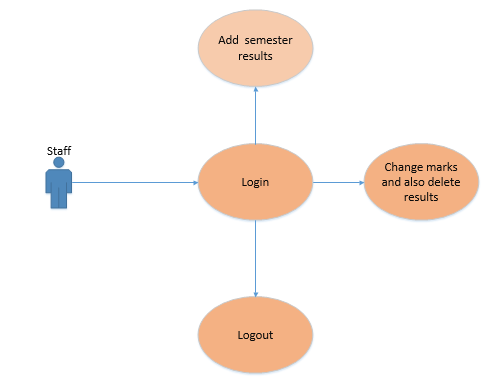
\includegraphics[trim={0cm 0cm 0cm 0cm },clip,scale = 1.1]{StaffUsecase}
\caption{Use Case Diagram For Staff}
\end{figure}
\end{center}



\begin{center}
    \begin{tabular}{ | p{2cm} | p{10cm}| }
    \hline
    \textbf{Use case}& \textbf{Description} \\ \hline
    login & Staff need to sign in order to modify results \\ \hline
    Change Results & Staff must be able to modify or add results  \\ \hline
    Logout          & Staff member must be able to logout  \\ \hline

    \end{tabular}
\end{center}




\clearpage
\subsubsection{Administrator Use-Case Report}$\;\;\;\;\;\;\;\;\;\;\;\;\;\;\;\;\;\;\;\;\;\;\;$

A use case report for an Administrator is shown in Figure 5.
\begin{center}
\begin{figure}[h]
\centering
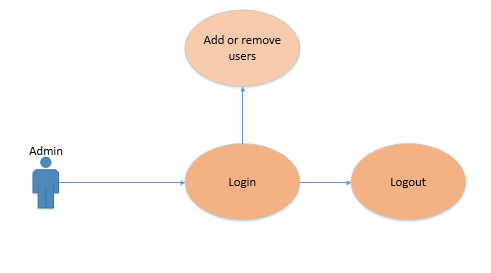
\includegraphics[trim={0cm 0cm 0cm 0cm },clip,scale = 1.1]{AdminUsecase}
\caption{Use Case Diagram For Administrator}
\end{figure}
\end{center}



\begin{center}
    \begin{tabular}{ | p{2cm} | p{10cm}| }
    \hline
    \textbf{Use case}& \textbf{Description} \\ \hline
    login & Administrator need to sign in \\ \hline
    Add users & The administrator must be able to add or remove users  \\ \hline
    Logout          & Administrator must be able to logout  \\ \hline

    \end{tabular}
\end{center}


\section{Sequence Diagram}

The sequence diagram in Figure 6 shows how each user interact with the interface and how the interface interact with database.  


\begin{center}
\begin{figure}[h]
\centering
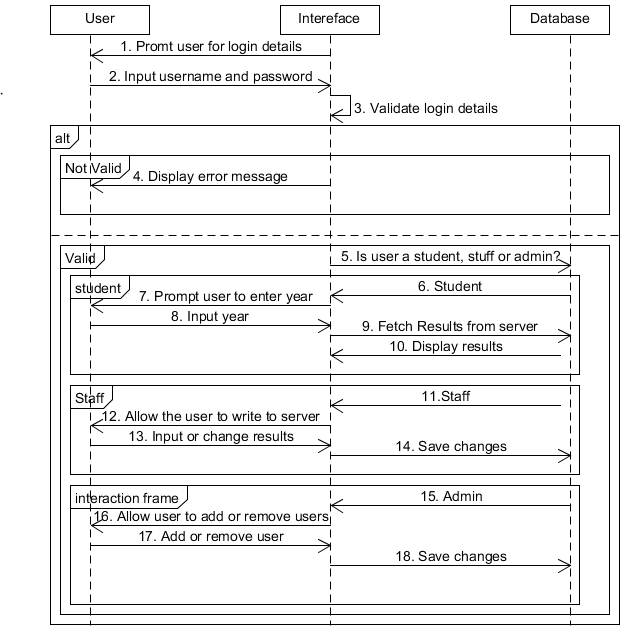
\includegraphics[trim={0cm 0cm 0cm 0cm },clip,scale = 1.1]{SequenceDig}
\caption{Sequence Diagram}
\end{figure}
\end{center}
\newpage

\vfill

%\nocite{*}
\bibliographystyle{witseie}
\bibliography{sample}

%{\tiny \vfill \hfill \today \hspace{5mm} witseie-paper-2003.\TeX}

\end{document}

" vim: ts=4
" vim: tw=78
" vim: autoindent
" vim: shiftwidth=4
